\chapter[Diziler ve Temel Teknikler · \textit{Temel}]{Diziler ve Temel Teknikler}
\chaptermark{Diziler ve Temel Teknikler}

Algoritmik problemlerin büyük bir kısmında veriler tek bir sayı veya değişken olarak değil, belirli bir sıra dahilinde peş peşe dizilmiş değerler topluluğu olarak karşımıza çıkar. Bir yarışmadaki katılımcıların puanları, bir hisse senedinin gün gün fiyatı ya da bir sensörden saniye saniye okunan sıcaklık değerleri bu duruma doğal birer örnektir. 

Bu bölümde, programlamanın en temel doğrusal veri yapısı olan dizileri ele alıyor; ardından zaman sınırına takılmamak için sıkça başvurulan iki temel tekniği inceliyoruz: \emph{prefix sums} (\emph{prefix sums}) ve \emph{two pointers} (\emph{two pointers}).

% =========================================================================
% BÖLÜM 1: DİZİLER, İNDİS, TARAMA
% =========================================================================
\section{Diziler, İndis ve Tarama}

\subsection{Motivasyon: Neden Dizi Kullanırız?}
Elinizde $5$ adet tam sayı olduğunu ve bunların ortalamasını bulmak istediğinizi varsayalım. Kolaylıkla $a, b, c, d, e$ adında beş değişken tanımlayıp toplamlarını $5$'e bölebilirsiniz. Peki ya $100\,000$ adet sayının ortalamasını, en büyüğünü veya sıralanmış halini bulmanız gerekirse? Yüz bin ayrı değişken ismi tanımlamak hem pratik değildir hem de algoritmik olarak anlamsızdır.

Bize gereken şey; bellekte art arda duran, tek bir isimle erişebildiğimiz ve her bir elemanına sırasıyla birer numara (indis) vererek ulaşabildiğimiz bir yapıdır. İşte bu yapıya \textbf{dizi} (\emph{array}) adı verilir.

\begin{definition}[Dizi ve İndis]
Aynı türden verilerin bellekte ardışık hücrelerde saklandığı, her bir elemanına $0$'dan (veya matematiksel yazımda $1$'den) başlayan bir tamsayı ile doğrudan erişilebilen veri yapısına \textbf{dizi} denir. Bir elemanın dizideki konumunu belirten bu tam sayıya \textbf{indis} (\emph{index}) adı verilir.
\end{definition}

Bir $A$ dizisinin $i$'inci elemanı programlamada genellikle \texttt{A[i]}, matematikte ise alt indisle $A_i$ veya $A[i]$ olarak gösterilir. C ve Python gibi dillerde dizilerin ilk elemanı daima $0$. indiste yer alır:
\[
A = [A_0, A_1, A_2, \dots, A_{n-1}]
\]

\subsection{Doğrudan Erişim ve Bellek Mantığı}
Dizilerin en belirgin avantajı, kaçıncı sırada olursa olsun herhangi bir elemana anında, yani $O(1)$ zamanda erişebilmesidir. 

Bellek mimarisinde her bir veri hücresinin bir adresi vardır. $n$ elemanlı bir tam sayı dizisi oluşturduğumuzda, işletim sistemi bellekte yan yana duran bloklar tahsis eder. İlk elemanın bellek adresi $\text{adres}_0$ ve her bir tam sayının kapladığı alan $w$ bayt (örneğin 32-bit tamsayılar için $w = 4$ bayt) ise, $i$'inci elemanın adresi şu formülle doğrudan hesaplanır:
\[
\text{adres}_i = \text{adres}_0 + i \times w
\]
İşlemci bu çarpma ve toplama işlemini tek bir makine çevriminde gerçekleştirir; aradaki elemanları tek tek saymak zorunda kalmaz. Bu nedenle $A[0]$'a erişmekle $A[99999]$'a erişmek aynı süreyi alır.

\subsection{Diziyi Döngüyle Gezme (Tarama)}
Dizi algoritmalarının temeli, elemanları belirli bir sıra ile incelemeye, yani \emph{tarama} (\emph{traversal}) işlemine dayanır. Bir diziyi baştan sona tek bir döngüyle geçtiğimizde, $n$ elemanın her birine tam bir kez uğrarız; bu da $O(n)$ karmaşıklık demektir.

\begin{example}
$n$ elemanlı bir $A$ tam sayı dizisindeki en büyük elemanı ve bu elemanın ilk görüldüğü indisi bulunuz.
\end{example}

\begin{proof}[Çözüm ve Düşünce Yolu]
Dizideki sayıları önceden bilmediğimiz için her sayıyı en az bir kez incelemek zorundayız. Karşılaştığımız en büyük değeri hafızada tutabiliriz. İlk başta gördüğümüz tek eleman olan $A[0]$'ı geçici olarak ``en büyük'' kabul ederiz. Ardından $1$'inci indisten son indise kadar diziyi sırayla gezeriz. Gezinti sırasında elimizdeki değeri aşan bir $A[i]$ ile karşılaşırsak, en büyük değeri ve indisini güncelleriz.

Bu işlem, Bölüm 18'de incelediğimiz \emph{yarı-değişmez} (\emph{monovariant}) mantığını taşır: $k$'ıncı adım tamamlandığında, elimizdeki değer $A[0 \dots k]$ alt dizisinin en büyük değeridir.

\begin{lstlisting}[language=CTemel]
int en_buyuk = A[0];
int en_buyuk_indis = 0;

for (int i = 1; i < n; i++) {
    if (A[i] > en_buyuk) {
        en_buyuk = A[i];
        en_buyuk_indis = i;
    }
}
\end{lstlisting}
Her adımda yalnızca sabit sayıda işlem ($O(1)$) yapıldığından ve döngü $n-1$ kez döndüğünden toplam zaman karmaşıklığı $O(n)$'dir.
\end{proof}

\begin{example}
Bir $A$ dizisinin kendi içinde tersine çevrilmesi (\emph{reverse}): Ek bir dizi kullanmadan, $A = [A_0, A_1, \dots, A_{n-1}]$ dizisini $A = [A_{n-1}, A_{n-2}, \dots, A_0]$ haline getiriniz.
\end{example}

\begin{proof}[Çözüm]
İlk eleman ($A[0]$) son elemanla ($A[n-1]$), ikinci eleman ($A[1]$) sondan bir öncekiyle ($A[n-2]$) yer değiştirmelidir. Genel kural olarak $i$'inci eleman $(n-1-i)$'inci elemanla takas edilir (\emph{swap}). 

Burada döngü sınırına dikkat edilmelidir: Dizinin sonuna kadar gidersek, ilk yarıda takas ettiğimiz elemanları ikinci yarıda tekrar takas edip eski hallerine döndürürüz. Dolayısıyla yalnızca dizinin ortasına ($\lfloor n/2 \rfloor$) kadar ilerlememiz yeterlidir:

\begin{lstlisting}
FUNCTION reverseArray(A)
    n = LENGTH(A)
    FOR i FROM 0 TO FLOOR(n / 2) - 1
        SWAP A[i] AND A[n - 1 - i]
    END FOR
END FUNCTION\end{lstlisting}
Döngü $\lfloor n/2 \rfloor$ adım attığı için zaman karmaşıklığı $O(n)$, ek bellek kullanımı ise $O(1)$'dir.
\end{proof}

\begin{example}[Frekans Dizisi / Sayma Tekniği]
Elemanları $0$ ile $K$ arasında değişen $n$ elemanlı bir dizide, her sayının kaçar kez tekrar ettiğini $O(n + K)$ zamanda bulunuz.
\end{example}

\begin{proof}[Çözüm]
İki iç içe döngü kurup her eleman için diziyi baştan sona taramak $O(n^2)$ zaman alırdı. Bunun yerine dizinin elemanlarını doğrudan birer \emph{indis} olarak kullanabiliriz. Boyutu $K+1$ olan ve tüm elemanları $0$'la başlatılmış bir \texttt{sayac} dizisi oluşturalım:

\begin{lstlisting}[language=CTemel]
// sayac dizisinin boyutu K + 1 olmali ve sifirlanmalidir
for (int i = 0; i < n; i++) {
    sayac[A[i]]++;
}
\end{lstlisting}
Bu işlemde her bir $A[i]$ için \texttt{sayac[A[i]]} değerini $1$ artırırız. Böylece tek bir taramayla ($O(n)$) tüm frekanslar belirlenmiş olur.
\end{proof}

\subsection*{En Sık Yapılan Hatalar: Sınır Taşması (Out-of-Bounds)}
Dizilerle çalışırken yarışmalarda en çok karşılaşılan ve programın anında çökmesine (Run Time Error) ya da tanımsız davranmasına (\emph{undefined behavior}) yol açan hata \textbf{indis sınır taşması}dır.
\begin{itemize}
    \item $n$ elemanlı bir dizide geçerli indisler $0, 1, \dots, n-1$'dir. \texttt{A[n]} indisine erişmeye çalışmak tipik bir ``bir fazlası hatası''dır (\emph{off-by-one error}).
    \item Komşu elemanları kontrol ederken (örneğin $A[i]$ ile $A[i+1]$ veya $A[i-1]$'i kıyaslarken) döngü sınırlarını daraltmayı unutmak: Döngü $i = 0$'dan $n-1$'e kadar dönüyorsa, döngü içinde $A[i+1]$ yazmak $i = n-1$ iken $A[n]$'e erişir ve taşma üretir.
\end{itemize}

% =========================================================================
% BÖLÜM 2: KÜMÜLATİF TOPLAMLAR (PREFIX SUMS)
% =========================================================================
\section{Prefix Sums}

\subsection{Motivasyon: Aralıksız Sorgular ve Zaman Çıkmazı}
Bir fabrikada çalışan bir makinenin $n$ gün boyunca harcadığı elektrik enerjisi bir $A$ dizisinde verilmiş olsun. Fabrika yönetimi sık sık şu soruyu yöneltiyor: ``$L$'inci gün ile $R$'inci gün arasında toplam ne kadar elektrik harcandı?''

Eğer bu soru toplam $q$ defa sorulursa ve biz her soru için $L$'den $R$'ye kadar olan sayıları bir döngü ile toplarsak ne olur?
\[
\text{Toplam} = \sum_{i=L}^{R} A[i]
\]
Her bir aralık sorgusu en kötü durumda $O(n)$ adım sürer. $q$ adet sorgu için harcanan toplam zaman $O(q \times n)$ olur. $n = 100\,000$ ve $q = 100\,000$ olan bir problemde işlem sayısı yaklaşık $10^{10}$ seviyesine ulaşır. Modern bir işlemci bir saniyede yaklaşık $10^8$ işlem yapabildiğinden, bu kaba kuvvet (\emph{brute-force}) yaklaşım $100$ saniye sürecek ve sınavdaki $1.0$ saniyelik zaman sınırını katbekat aşacaktır.

Dizideki sayılar sabitken her seferinde aynı aralıkları tekrar tekrar toplamak yerine bu toplamları önceden hazırlayabiliriz.

\subsection{Sezgi ve Genel Kural}
Somut bir örnek üzerinden düşünelim. Bir yol üzerinde $0$'ıncı kilometreden başlayarak ilerleyen bir aracın belirli noktalardaki kilometre taşlarını biliyor olalım:
\[
A = [3, \, 1, \, 4, \, 1, \, 5, \, 9, \, 2]
\]
Bu aracın $2$. eleman ile $5$. eleman arasındaki (yani $4, 1, 5, 9$) mesafesini bulmak istiyoruz. 

Yolun en başından itibaren gidilen toplam mesafeleri önceden kaydetmiş olsaydık:
\begin{itemize}
    \item Baştan $5$. elemana kadar olan toplam mesafe: $3 + 1 + 4 + 1 + 5 + 9 = 23$
    \item Baştan $1$. elemana kadar olan toplam mesafe: $3 + 1 = 4$
\end{itemize}
Aradığımız $[2, 5]$ aralığı, aslında ilk $5$ elemanın toplamından ilk $1$ elemanın toplamının çıkarılmasıyla bulunur:
\[
\text{Aralık Toplamı} = 23 - 4 = 19
\]
Kontrol edelim: $4 + 1 + 5 + 9 = 19$. Tek bir çıkarma işlemiyle sonuca ulaştık.

\begin{definition}[Prefix Sums Dizisi]
Boyutu $n$ olan bir $A$ dizisi verildiğinde, $P[0] = 0$ olmak üzere her $1 \le k \le n$ için
\[
P[k] = \sum_{i=0}^{k-1} A[i] = A[0] + A[1] + \dots + A[k-1]
\]
şeklinde tanımlanan $n+1$ elemanlı $P$ dizisine $A$'nın \textbf{prefix sum dizisi} (\emph{prefix sum array}) denir.
\end{definition}

\textbf{Notasyon ve $1$-Tabanlı Tercih:} Prefix sums dizilerinde $P$'nin boyutunu $n+1$ seçip $P[0] = 0$ tanımlamak büyük bir indeksleme kolaylığı sağlar. Böylece ilk $k$ elemanın toplamı doğrudan $P[k]$ olur.

\begin{theorem}[Aralık Toplamı İlkesi]
$0$-tabanlı indekslenmiş bir $A$ dizisinin $[L, R]$ indis aralığındaki elemanlarının toplamı, $P$ prefix sum dizisi kullanılarak $O(1)$ zamanda şu formülle hesaplanır:
\[
\sum_{i=L}^{R} A[i] = P[R+1] - P[L]
\]
\end{theorem}

\begin{proof}
Tanım gereği:
\[
P[R+1] = A[0] + A[1] + \dots + A[L-1] + A[L] + \dots + A[R]
\]
ve
\[
P[L] = A[0] + A[1] + \dots + A[L-1]
\]
dir. İki eşitliği taraf tarafa çıkardığımızda:
\[
P[R+1] - P[L] = \left(\sum_{i=0}^{R} A[i]\right) - \left(\sum_{i=0}^{L-1} A[i]\right) = \sum_{i=L}^{R} A[i]
\]
elde edilir. Bu hesaplama yalnızca tek bir çıkarma işleminden ibaret olduğundan çalışma zamanı $O(1)$'dir.
\end{proof}

\subsection{Prefix Sums İnşası}
$P$ dizisini her adımda baştan toplayarak kurarsak inşa süreci $O(n^2)$ sürer. Ancak bir önceki toplamı kullanarak yeni elemanı eklemek doğal bir yineleme verir:
\[
P[i] = P[i-1] + A[i-1] \quad (1 \le i \le n)
\]
Bu ilişki sayesinde $P$ dizisi $O(n)$ zamanda, tek bir geçişte kurulur.

\begin{lstlisting}[language=CTemel]
// A dizisi n elemanli, P dizisi n + 1 elemanli
P[0] = 0;
for (int i = 1; i <= n; i++) {
    P[i] = P[i - 1] + A[i - 1];
}

// L ile R araligindaki toplami sorgulamak icin (0 <= L <= R < n):
long long aralik_toplami = P[R + 1] - P[L];
\end{lstlisting}

Böylece $q$ sorguluk problemimizin toplam süresi $O(q \times n)$ yerine $O(n + q)$ olur ve sorgular hızla yanıtlanır.

\begin{example}
Sıfırlardan ve birlerden oluşan bir dizide, verilen $[L, R]$ aralığında kaç tane \texttt{\$1\$} olduğunu $O(1)$ zamanda bulan algoritmayı tasarlayınız.
\end{example}

\begin{proof}[Çözüm]
Yalnızca $0$ ve $1$'lerden oluşan bir dizide elemanların toplamı, dizideki $1$'lerin sayısına tam olarak eşittir. Dolayısıyla dizinin prefix sumını aldığımızda, herhangi bir $[L, R]$ aralığındaki $1$'lerin sayısı doğrudan $P[R+1] - P[L]$ formülüyle elde edilir.
\end{proof}

\begin{example}[Toplamı $K$ Olan Alt Dizi Sayısı]
Negatif sayılar da içerebilen $n$ elemanlı bir $A$ dizisinde, toplamları tam olarak $K$'ya eşit olan ardışık alt dizilerin sayısını bulunuz. ($n \le 200\,000$)
\end{example}

\begin{proof}[Çözüm ve Düşünce Yolu]
Bu fikir şuradan gelir: Bir $[L, R]$ alt dizisinin toplamı $P[R+1] - P[L]$'dir. Bizden istenen koşul:
\[
P[R+1] - P[L] = K \iff P[L] = P[R+1] - K
\]
Bu matematiksel dönüşüm çözümü oldukça sadeleştirir. Diziyi soldan sağa doğru tararken ($R$'yi $0$'dan $n-1$'e büyütürken), o ana kadar gördüğümüz prefix sums'ın frekansını bir tabloda saklarsak; her adımda ``Geçmişte değeri $P[R+1] - K$ olan kaç tane $P[L]$ gördüm?'' sorusunu doğrudan yanıtlayabiliriz:

\begin{enumerate}
    \item \texttt{toplam\_adet = 0}, \texttt{suanki\_toplam = 0}.
    \item Boş bir frekans tablosu açıp \texttt{frekans[0] = 1} yazarız (hiç eleman almadığımız boş önek toplamı $0$'dır).
    \item Dizinin her $x$ elemanı için:
    \begin{itemize}
        \item \texttt{suanki\_toplam += x}
        \item Aradığımız eski değer \texttt{hedef = suanki\_toplam - K}.
        \item Eğer \texttt{hedef} tabloda varsa, \texttt{toplam\_adet += frekans[hedef]}.
        \item \texttt{frekans[suanki\_toplam]} değerini $1$ artır.
    \end{itemize}
\end{enumerate}
Bu algoritma diziyi tek bir geçişte, $O(n)$ sürede çözer.
\end{proof}

\subsection{İki Boyutlu Prefix Sums}
Prefix sums mantığı çok boyutlu dizilere de doğrudan genellenir. $H \times W$ boyutlarında bir matriste verilen herhangi bir dikdörtgensel bölgenin toplamını $O(1)$ sürede bulmak için benzer bir önek hesabı kurulabilir.

\begin{definition}[2 Boyutlu Prefix Sums]
$M$ matrisi için $P[r][c]$, sol üst köşesi $(0, 0)$ ve sağ alt köşesi $(r-1, c-1)$ olan dikdörtgenin içindeki tüm sayıların toplamıdır.
\end{definition}

Bunu hesaplarken Bölüm 8'de ele aldığımız içerme-dışarma ilkesinden (\emph{inclusion-exclusion}) faydalanırız:
\[
P[r][c] = M[r-1][c-1] + P[r-1][c] + P[r][c-1] - P[r-1][c-1]
\]
Solundaki ve üstündeki alanlar toplanır; her ikisinde de ortak bulunan sol-üst çapraz alan iki kez sayıldığı için bir kez çıkarılır.

Benzer şekilde, sol üst köşesi $(r_1, c_1)$ ve sağ alt köşesi $(r_2, c_2)$ olan bir alt matrisin toplamı şudur:
\[
\text{Alan Toplamı} = P[r_2+1][c_2+1] - P[r_1][c_2+1] - P[r_2+1][c_1] + P[r_1][c_1]
\]

\begin{figure}[h]
\centering
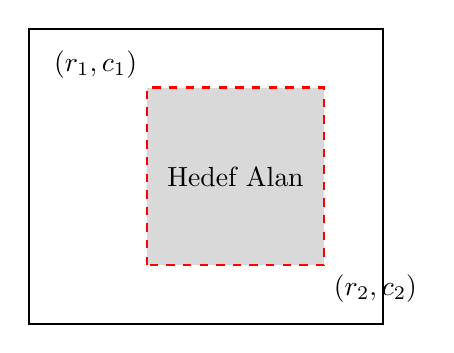
\begin{tikzpicture}[scale=0.75]
    % Büyük dikdörtgen
    \draw[thick] (0,0) rectangle (6,5);
    % Alt bölgeler
    \fill[gray!30] (2,1) rectangle (5,4);
    \draw[dashed, red, line width=1pt] (2,1) rectangle (5,4);
    \node at (3.5, 2.5) {Hedef Alan};
    \node[above left] at (2,4) {$(r_1, c_1)$};
    \node[below right] at (5,1) {$(r_2, c_2)$};
\end{tikzpicture}
\caption{2 Boyutlu Prefix Sums'ta Hedef Alanın İçerme-Dışarma ile Hesaplanması}
\end{figure}

\subsection{Fark Dizisi Tekniği (Difference Array)}
Prefix sums'ın ters işlemi de aralık güncellemelerinde oldukça etkilidir. Diyelim ki boş bir diziyle başladınız ve size şu tip güncellemeler veriliyor: ``$[L, R]$ aralığındaki tüm sayılara $V$ değerini ekle.''

$q$ adet aralık güncellemesini döngüyle yapmak $O(q \times n)$ sürer. Ancak \textbf{fark dizisi} tekniğiyle her güncellemeyi $O(1)$ işlemle kaydedebiliriz:

$D$ fark dizisi, $D[i] = A[i] - A[i-1]$ olarak tanımlansın ($A[-1]=0$). $[L, R]$ aralığına $V$ eklemek, fark dizisinde yalnızca iki noktayı etkiler:
\begin{enumerate}
    \item $D[L]$ değeri $V$ kadar artar ($A[L]$, $A[L-1]$'e kıyasla $V$ kadar büyümüştür).
    \item $D[R+1]$ değeri $V$ kadar azalır ($A[R+1]$ değişmemiş, ancak solundaki $A[R]$ değeri $V$ kadar büyümüştür).
\end{enumerate}

Tüm sorgular bittikten sonra, fark dizisinin prefix sumı alınarak orijinal dizinin son hali tek hamlede $O(n)$ sürede elde edilir.

\subsection*{En Sık Yapılan Hatalar}
\begin{itemize}
    \item \textbf{Tamsayı Taşması (Integer Overflow):} Dizi elemanları $10^9$ mertebesindeyse, bu elemanların toplamı 32-bit işaretli tamsayı sınırını ($2^{31}-1 \approx 2 \times 10^9$) hızla aşar. Prefix sums dizisi tanımlanırken C/C++ dillerinde mutlaka \texttt{long long} türü tercih edilmelidir.
    \item \textbf{İndis Kaymaları:} $P[R] - P[L]$ mi yoksa $P[R+1] - P[L]$ mi yazılacağı sıkça karıştırılır. Sağlamasını yapmak için $1$ elemanlı bir aralığı ($L = R$) test edebilirsiniz: Formülün $P[L+1] - P[L] = A[L]$ sonucunu vermesi gerekir.
\end{itemize}

% =========================================================================
% BÖLÜM 3: İKİ İŞARETÇİ (TWO POINTERS)
% =========================================================================
\section{Two Pointers}

\subsection{Motivasyon: Sıralı Yapıların Getirdiği Bilgi Gücü}
Elimizde küçükten büyüğe sıralanmış bir $A$ dizisi olsun:
\[
A = [1, \, 3, \, 4, \, 7, \, 10, \, 11, \, 15], \quad n = 7
\]
Bu dizide toplamları tam olarak $X = 17$ olan iki eleman bulmak istiyoruz.

Akla gelen ilk yöntem, iç içe iki döngü yazıp tüm olası $(A[i], A[j])$ çiftlerini denemektir. Olası çift sayısı $\binom{n}{2} = \frac{n(n-1)}{2} = O(n^2)$'dir. $n = 100\,000$ durumunda bu yaklaşım zaman aşımına uğrar.

Dizinin \textbf{sıralı} olması ise bize net bir yön bilgisi verir: Sağa gitmek sayıları büyütür, sola gitmek küçültür. Bu sayede arama uzayını körlemesine denemek yerine adım adım daraltabiliriz.

\subsection{Uçlardan Merkeze Tarama (Opposite Direction)}
Diziye iki uçtan yaklaşalım: Biri dizinin en küçük elemanını (en başı, $sol = 0$), diğeri ise en büyük elemanını (en sonu, $sag = n - 1$) göstersin. Konum belirten bu değişkenlere \textbf{işaretçi} (\emph{pointer}) diyoruz.

\begin{figure}[h]
\centering
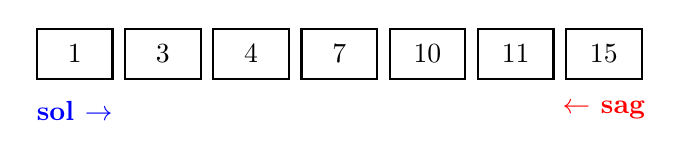
\begin{tikzpicture}[scale=0.8]
    \foreach \x/\val in {0/1, 1/3, 2/4, 3/7, 4/10, 5/11, 6/15} {
        \draw[thick] (\x*1.4, 0) rectangle (\x*1.4+1.2, 0.8);
        \node at (\x*1.4+0.6, 0.4) {$\val$};
    }
    \node[below, blue, font=\bfseries] at (0.6, -0.2) {sol $\rightarrow$};
    \node[below, red, font=\bfseries] at (6*1.4+0.6, -0.2) {$\leftarrow$ sag};
\end{tikzpicture}
\caption{Two Pointers Yaklaşımında İşaretçilerin İki Uçtan Başlatılması}
\end{figure}

Şimdi mevcut toplama bakalım: $T = A[sol] + A[sag] = 1 + 15 = 16$.
\begin{itemize}
    \item Aradığımız toplam $17$'ydi; mevcut toplam ($16$) küçük kaldı.
    \item Toplamı büyütmek için $sag$ işaretçisini sola kaydırırsak sayılar küçülür ve toplam daha da azalır. Dolayısıyla $A[sag]$ ile eşleşebilecek başka hiçbir eleman kalmamıştır. Toplamı büyütmenin tek yolu $sol$ işaretçisini bir adım sağa ilerletmektir ($sol = 1$).
\end{itemize}

Yeni durum: $A[sol] = 3$, $A[sag] = 15$. Toplam $3 + 15 = 18$.
\begin{itemize}
    \item Bu sefer toplam hedefimizden büyük çıktı ($18 > 17$).
    \item Toplamı küçültmek için $sag$ işaretçisini bir adım sola kaydırmalıyız ($sag = 5$).
\end{itemize}

Yeni durum: $A[sol] = 3$, $A[sag] = 11$. Toplam $3 + 11 = 14 < 17$. $sol$ bir sağa ($sol = 2$).\\
Yeni durum: $A[sol] = 4$, $A[sag] = 11$. Toplam $4 + 11 = 15 < 17$. $sol$ bir sağa ($sol = 3$).\\
Yeni durum: $A[sol] = 7$, $A[sag] = 11$. Toplam $7 + 11 = 18 > 17$. $sag$ bir sola ($sag = 4$).\\
Yeni durum: $A[sol] = 7$, $A[sag] = 10$. Toplam $7 + 10 = 17 = X$. Aradığımız çifti bulduk: $(7, 10)$.

\begin{theorem}[Two Pointers ile İki Toplam (Two Sum)]
Küçükten büyüğe sıralı $n$ elemanlı bir dizide toplamı $X$ olan bir çiftin varlığı, two pointers tekniği ile $O(n)$ zamanda ve $O(1)$ ek bellek ile tespit edilebilir.
\end{theorem}

\begin{proof}[İspat ve Değişmez (Invariant)]
Algoritmanın doğruluğunu göstermek için aradığımız çözümün adımlar sırasında elenmediğini kanıtlamalıyız.

Aranan çözümün $(i^*, j^*)$ indislerinde bulunduğunu varsayalım ($i^* < j^*$). Bölüm 18'de ele aldığımız değişmezlik yaklaşımıyla, ispatlamak istediğimiz \emph{değişmez} şudur: ``Herhangi bir anda $sol \le i^*$ ve $sag \ge j^*$ eşitsizlikleri daima korunur.''

Başlangıçta $sol = 0 \le i^*$ ve $sag = n-1 \ge j^*$ olduğundan ifade geçerlidir. Algoritmanın adımlarında iki durum oluşabilir:
\begin{enumerate}
    \item $A[sol] + A[sag] < X$: Eğer $sol < i^*$ ise, $sol$'un bir artması aradığımız $i^*$'a doğru yaklaşmadır; değişmez bozulmaz. $sol = i^*$ iken bu durum gerçekleşebilir mi? Gerçekleşemez; çünkü $sol = i^*$ olsaydı, $sag \ge j^*$ koşulundan ötürü $A[sol] + A[sag] = A[i^*] + A[sag] \ge A[i^*] + A[j^*] = X$ olurdu. Bu ise toplamın $X$'ten küçük olmasıyla çelişir. Dolayısıyla $sol = i^*$ iken işaretçi artırılmaz.
    \item $A[sol] + A[sag] > X$: Benzer şekilde $sag = j^*$ iken toplam asla $X$'ten büyük olamaz. Dolayısıyla $sag$, hiçbir zaman $j^*$'ın soluna düşecek şekilde eksiltilmez.
\end{enumerate}
İşaretçilerden en az biri her adımda diğerine bir birim yaklaşır ($sag - sol$ farkı kesin olarak azalır). Dolayısıyla algoritma en fazla $n$ adımda ya hedef çifte ulaşır ya da $sol \ge sag$ koşuluyla sonlanır. Toplam işlem sayısı $O(n)$'dir.
\end{proof}

\begin{lstlisting}[language=CTemel]
int sol = 0, sag = n - 1;
bool bulundu = false;

while (sol < sag) {
    long long toplam = (long long)A[sol] + A[sag];
    if (toplam == X) {
        bulundu = true;
        break;
    } else if (toplam < X) {
        sol++; // Toplami buyut
    } else {
        sag--; // Toplami kucult
    }
}
\end{lstlisting}

\subsection{Aynı Yöne Kayan Pencere (Sliding Window)}
İki işaretçinin her zaman dizinin iki zıt ucundan başlaması gerekmez. Kimi problemlerde two pointers de dizinin başından ($0$'dan) başlar ve aynı yöne doğru ilerler. Bu yaklaşıma \textbf{kayan pencere} (\emph{sliding window}) denir. Pencerenin sınırlarını $[sol, sag]$ aralığı belirler.

\begin{example}[Toplamı En Fazla $K$ Olan En Uzun Alt Dizi]
Tüm elemanları \textbf{pozitif} tam sayılar olan bir $A$ dizisinde, elemanları toplamı $\le K$ olan en uzun ardışık alt dizinin uzunluğunu bulunuz.
\end{example}

\begin{proof}[Çözüm ve Düşünce Yolu]
Tüm elemanlar pozitif olduğu için penceremize sağdan yeni bir eleman eklediğimizde ($sag$ arttığında) toplam kesinlikle \emph{artar}; soldan bir eleman çıkardığımızda ($sol$ arttığında) toplam kesinlikle \emph{azalır}. Bu durum arama için elverişli bir monotonluk sunar.

$sag$ işaretçisini $0$'dan $n-1$'e kadar birer birer ilerletiriz. Her adımda $A[sag]$'ı pencere toplamına ekleriz. Eğer toplam $K$'yı aşarsa, toplam tekrar $K$'nın altına inene kadar $sol$ işaretçisini sağa kaydırıp $A[sol]$ değerlerini pencereden çıkarırız:

\begin{lstlisting}
FUNCTION longestSubarray(A, K)
    left = 0
    currentSum = 0
    maxLength = 0

    FOR right FROM 0 TO length(A) - 1 DO
        currentSum = currentSum + A[right]

        WHILE currentSum > K AND left <= right DO
            currentSum = currentSum - A[left]
            left = left + 1
        END WHILE

        maxLength = MAX(maxLength, right - left + 1)
    END FOR

    RETURN maxLength
END FUNCTION\end{lstlisting}

\textbf{Karmaşıklık Analizi (Amorti Edilmiş Analiz):} 
Kodda iç içe bir \texttt{for} ve bir \texttt{while} döngüsü yer alması ilk bakışta $O(n^2)$ izlenimi verebilir. Ancak işaretçilerin hareketine dikkat edilmelidir: 
\begin{itemize}
    \item $sag$ işaretçisi $0$'dan $n-1$'e kadar tam $n$ defa artırılır.
    \item $sol$ işaretçisi hiçbir zaman sola dönmez; o da dizi boyunca en fazla $n$ defa artırılabilir.
\end{itemize}
Dolayısıyla içteki \texttt{while} döngüsünün toplam adım sayısı, programın tüm çalışma süresi boyunca en fazla $n$'dir. Amorti edilmiş analizle her eleman pencereye bir kez girer ve en fazla bir kez çıkar. Toplam zaman karmaşıklığı $O(n)$'dir.
\end{proof}

\begin{example}[Sıralı İki Diziyi Birleştirme / Merge]
Boyutları sırasıyla $n$ ve $m$ olan sıralı iki dizi $A$ ve $B$ verildiğinde; bu iki diziyi tek bir sıralı dizi halinde $O(n+m)$ zamanda birleştiriniz.
\end{example}

\begin{proof}[Çözüm]
Bu problem, Bölüm 23'te göreceğimiz Birleştirmeli Sıralama (\emph{Merge Sort}) algoritmasının temel adımıdır. $A$ için bir $i$ işaretçisi, $B$ için bir $j$ işaretçisi tutarız. Her adımda $A[i]$ ve $B[j]$'den hangisi daha küçükse onu yeni dizimize ekler ve ilgili işaretçiyi bir ilerletiriz:

\begin{lstlisting}[language=CTemel]
int i = 0, j = 0, k = 0;
// C dizisi (n + m) boyutundadir
while (i < n && j < m) {
    if (A[i] <= B[j]) {
        C[k++] = A[i++];
    } else {
        C[k++] = B[j++];
    }
}
// Kalan elemanlari aktar
while (i < n) C[k++] = A[i++];
while (j < m) C[k++] = B[j++];
\end{lstlisting}
Her adımda bir işaretçi ilerlediğinden toplam zaman $O(n+m)$ olur.
\end{proof}

\subsection*{En Sık Yapılan Hatalar: Negatif Sayılar ve Monotonluk İhlali}
Kayan pencere (veya two pointers) tekniğinin çalışabilmesi için sistemde bir \textbf{monotonluk} (tekdüzelik) bulunması şarttır. Örneğin ``Toplamı $\le K$ olan alt dizi'' probleminde dizide \textbf{negatif sayılar da yer alsaydı}, pencereye sağdan eleman eklemek toplamı küçültebilir, soldan eleman çıkarmak toplamı büyütebilirdi. Bu durumda işaretçilerin hangi yönde ilerletilmesi gerektiği kestirilemez ve two pointers tekniği geçerliliğini yitirir.

\textbf{Altın Kural:} Negatif sayıların bulunduğu toplam problemlerinde two pointers yerine yukarıda incelediğimiz \emph{prefix sum + frekans tablosu} yöntemi tercih edilmelidir.

% =========================================================================
% BÖLÜM ÖZETİ VE REHBER
% =========================================================================
\section*{Bölüm Özeti ve Hangi Tekniği Seçmeli?}

TÜBİTAK 1. Aşama sınavında bir dizi problemiyle karşılaştığınızda şu karar ağacı yol gösterici olabilir:

\begin{enumerate}
    \item \textbf{Tekrarlı Aralık Sorguları (Range Queries):} Dizi sabit kalıyor ve bize defalarca $[L, R]$ aralığındaki toplam, çift sayı adedi vb. soruluyorsa $\rightarrow$ \textbf{Prefix Sums ($O(1)$ sorgu)}.
    \item \textbf{Toplu Aralık Güncellemeleri (Range Updates):} Birden fazla aralığa sabit bir değer eklenip en sonunda dizinin nihai hali isteniyorsa $\rightarrow$ \textbf{Fark Dizisi ($O(1)$ güncelleme)}.
    \item \textbf{Sıralı Dizide Eşleşme / Çift Arama:} Dizi sıralıysa (veya sıralanabiliyorsa) ve belirli bir toplamı/farkı sağlayan eleman çifti aranıyorsa $\rightarrow$ \textbf{Zıt Yönlü İki İşaretçi ($O(n)$)}.
    \item \textbf{Pozitif Değerli Dizilerde Alt Dizi Optimizasyonu:} Elemanların pozitif olduğu ve bir aralık koşulunun (örneğin toplam $\le K$) arandığı sorularda $\rightarrow$ \textbf{Kayan Pencere ($O(n)$)}.
\end{enumerate}
